\chapter{Construction of the multiband catalog over Stripe 82}\label{CH_02}

	SED fitting requires supplying catalogs that contains multi-wavelength photometry. Quality of photometric data is very important for proper estimation of the properties of the galaxies. In this chapter we shall describe our strategy for construction of such catalogs, optical and IR, general issues that arise and our methods to solve it.
	
	SDSS co-adds from J14 that we utilize already have catalogs on the whole Stripe 82 region. We decide not to use it and create our own catalogs for several reasons:\\
	-	The catalogs are not matched between the bands, resulting in different object lists for each band within the same region,so there may be misidentification of the sources when we attempt to construct multiband catalog with data from all 5 bands.\\
	-	SNR at which the source is rejected from the catalog was chosen too high and there are a lot of sources that we shall use, which are not included in J14 catalog.\\
	-	Bright and saturated objects are generally represented in this catalog as multiple sources, none of which is at the center of such object. This means that when SED fitting is performed for this source, non-physical stellar mass and redshifts will be produced. \\
	On Figure~\ref{fig:catalog_comp} we present a comparison of the original catalog from J14 (sources within green regions) and our catalog, that was constructed independently (sources within red regions) and will be presented further in this chapter.
	
\begin{figure}[!ht]
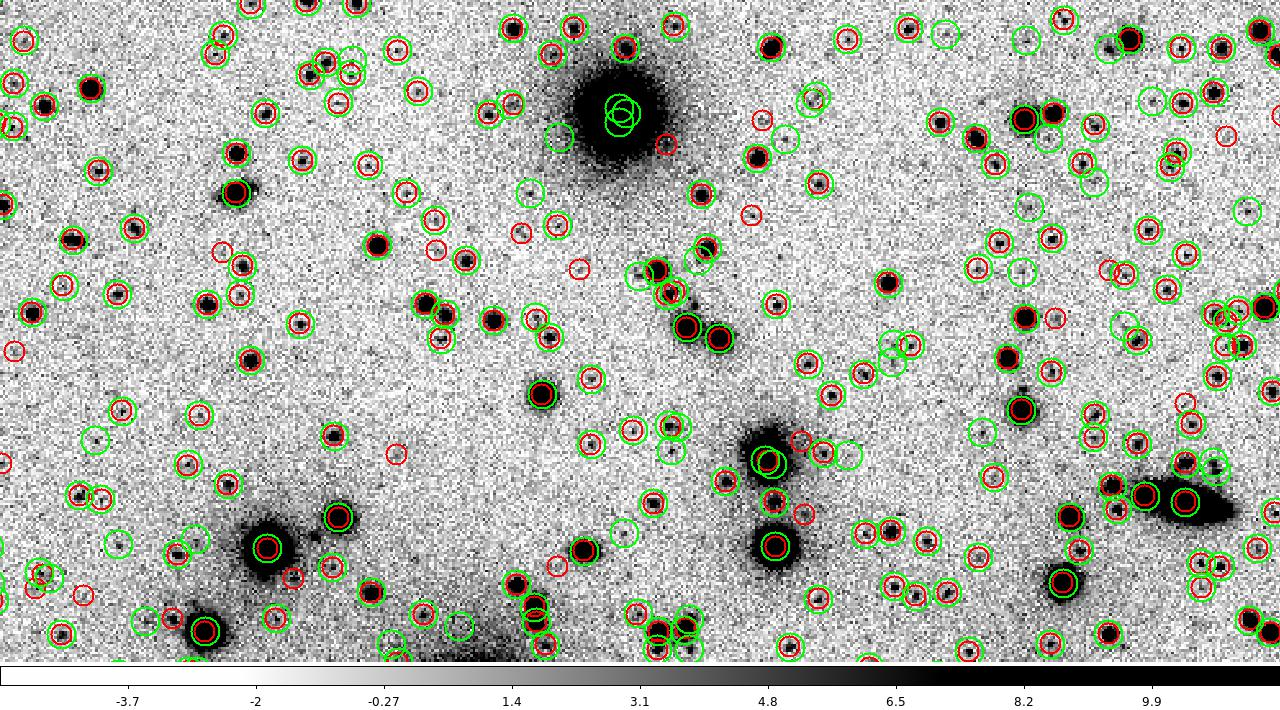
\includegraphics[width=6in]{Figures/catalog_comparison.jpeg}
\caption{Optical catalogs from J14 (green circles) and our catalog (red circles) are overplotted on a small random area in Stripe 82. There is a number of well-detected sources that were excluded from J14 catalog and also there are multiple detections around a saturated source in the upper part of the plot. Our catalog aims to resolve both such issues.}
\label{fig:catalog_comp}
\end{figure}	
	
	
	The most critical factor in the success of this project is consistent photometry from optical to near-IR. This is challenging because the spatial resolutions of WISE is $\sim$5-6x worse than that of SDSS. For this reason, the objects detected in WISE often suffer blending. Even for relatively isolated WISE sources, the photometric apertures appropriate for the (low resolution) WISE images cannot guarantee the same fraction of light being included as what is done in the (high resolution) SDSS images. Such a systematic offset, which is different for every galaxy of different morphology, can severely skew the SED fitting.

To best address this problem, we opt to use the {\tt TPHOT} software \citep{Merlin2016a}, which recently emerged as a robust and flexible tool to perform $"$template fitting$"$. The basic idea is to use a high-resolution image (here SDSS) as the prior to build the morphological template of the source under question, convolve this template with the PSF of the low-resolution image (here WISE), and fit this degraded template to the low-resolution image to obtain the total flux that is within the aperture as defined by the high-resolution image. In this way, we get reliable color information (i.e., flux ratio) in the most consistent manner. It is important to note that high-resolution source does not have to be point-like - its morphological features will be preserved and fitted to the low-resolution source. This implies the biggest assumption for this technique - that morphology of the source is wavelength-independent. While generally it is not true, especially for the actively star-forming or dusty galaxies, we anticipate that this will not create any significant bias. Firstly, because most of the galaxies have small angular sizes and such variation in sizes is small (galaxy at z=0.7 that is 40 kpc in diameter has an angular size of only 6 pixels), and secondly, because we chose SDSS r-band ($6202.46~\AA$), that is a red filter, as a high-resolution image - there should not be much morphological difference between r-band and w1 or w2 bands..\\

Proper use of {\tt TPHOT} requires several preliminary operations with both high- and low-resolution images, and construction of optical catalogs also consists of a number of steps. It is impossible to separate operations for these two main stages - chronologically the steps for both stages are intermixed. In the following sections we shall describe general algorithm in the order in which it was implemented in the project.

\section{Preparatory work with SDSS images and optical catalog}
	
	High-resolution optical image is used not only to determine flux and morphology of the source in near-IR, but also its position. For that reason high- and low-resolution images should have the same type of projection, reference coordinate and orientation written in their FITS headers \citep{Pence2010}. SDSS and WISE images have the same tangential projection and orientation ($CD1\_2=0$, $CD2\_1=0$), so we leave these values unchanged. Each WISE frame covers $\approx 3.95 deg^{2}$ and there may be up to 72 SDSS images that cover the same area, so we decide to use coordinates of the center of WISE images (CRVAL1 and CRVAL2) as the anchor values and run {\tt SWarp} \citep{Bertin2002} to change reference pixels in all SDSS images. The reference pixel (CRPIX1 and CRPIX2) for SDSS images can now be outside of the image itself to as far as 0.7 deg. 
	
\subsection{Region of overlapping unWISE images}

Some SDSS images may reside on the border between two overlapping unWISE images. In such a case 2 copies of SDSS image are created, each is processed by {\tt SWarp} independently, gets its own set of CRPIX and CRVAL values and from now on is treated separately. 
The following example shows the current naming convention that is used throughout this work: $S82\_3282m016\_01r\_097.fits$ and $S82\_3297m016\_01r\_097.fits$ means that original image $S82\_01r\_097.fits$ now has two sets of CRVAL values - one is the same as the coordinates of the center of image unwise-3282m016-w1-img-m.fits and the other - of image unwise-3297m016-w1-img-m.fits.

This "duplication" increased the number of SDSS images in each band from 4,812 to 5,556.
	
\subsection{SDSS PSF construction}
	Optical part of the catalog consists of 5 SDSS bands, each of which has different sensitivity and FWHM, so each field has different number of sources in different bands. We shall choose the band that we use for detection, i.e., the source is added to our catalog if only it is detected in this band with sufficient SNR. Also position of the source in this band is used as the true position in all other bands. Another issue is the flux measurement - reliable SED fitting requires consistent multiwavelength photometry while different photometric conditions and FWHM could result in a non-consistent colors even in optical filters alone. Thus the measurment that are made even with flexible elliptical apertures known as the Kron apertures \citep{Kron1980} that are denoted  in {\tt SExtractor} as FLUX\_AUTO \citep{Bertin1996} will not be measuring the same fraction of the total flux from the given source in different filters. We decided to convolve \textit{griz} bands to the one with the worst FWHM, i.e., u-band. In such case the difference in sizes will be due to the intrinsic difference in morphology at different wavelength rather than due to difference in optics. For the price of loosing some sources due to blending we shall achieve better consistency in our optical colors. We use {\tt IRAF/psfmatch} task that requires supplying the image with the corresponding kernel - PSF matching function to be convolved with the input image to produce the output one. Construction of a kernel requires a knowledge of the PSFs of the input image and a matched image. That means we need to construct PSF for each image in each band ($5,556\cdot 5 = 27,780$ PSFs) and this is the most time-consuming part of the project.

One of the widely-used ways to construct a PSF is using {\tt PSFEx} software \citep{Bertin2011}. We tested it with {\tt TPHOT} and found that the quality of residual images is not satisfactory, so we decided to use more conservative algorithm in which {\tt IRAF/psf} task creates a PSF function based on a set of selected point-like sources (so called PSF stars). Usually that strategy involves consecutive run of {\tt IRAF/find}, {\tt IRAF/phot}, {\tt IRAF/pstselect} and {\tt IRAF/psf} tasks that find stars, determine its magnitude, select the ones that do not have any morphological features and finally construct a PSF function. This algorithm, though much more reliable, is also not ideal - in each image there are $\sim 10\% $ of sources that do not satisfy the criteria of PSF stars (are elongated, blended or have noisy background) and have to be rejected in the manual regime (selection in interactive mode). This is extremely time-consuming and inefficient given the total number of images in 5 bands. We decide to use a variation of this method to create PSF functions in a more automatic fashion that is presented in the next passage. 

We run {\tt SExtractor} on each SDSS image and only mark sources from the output catalog as a point-like, if their "stellarity" index (determined by a CLASS\_STAR parameter) is close to 1, sources are bright, but not saturated, do not lay within $2 \cdot PSF~radius$ to the edge of the FITS image, and have all their flux contained within some small aperture. The later was confirmed by finding the difference "MAG diff" between MAG\_APER that returns all flux within some fixed aperture and MAG\_BEST that returns MAG\_AUTO value in the absence of contamination from the nearby sources and MAG\_ISOCOR otherwise. Exact parameters depend on the band and also were adjusted during test runs so that each SDSS image has no less than 20 PSF stars (stars were sorted by their magnitude, from bright to dim), with the maximum number of PSF stars limited to 160 (larger values significantly slow down {\tt IRAF}). Selection criteria can be found in Table~\ref{tab:psf_star}

\begin{table}[h!]
  \begin{center}
    \caption{Table of parameters for selection of PSF stars}
    \label{tab:psf_star}
    \begin{tabular}{l|l|l|l|l|l} % <-- Changed to S here.
      \textbf{parameter} & \textbf{u} & \textbf{g} & \textbf{r} & \textbf{i} & \textbf{z}\\
%      $\alpha$ & $\beta$ & $\gamma$ \\
      \hline
%      aperture [pix]  & ?? & ?? & ?? & ?? & ??\\
      MAG diff & -0.06 -- -0.14 & -0.04 -- -0.1 & -0.1 -- 0.7 & -0.1 -- 0.7 & -0.1 -- 0.7\\
      CLASS\_STAR min & 0.80 & 0.85 & 0.85 & 0.85 & 0.80\\
      MAG\_AUTO min   & 13.5 & 13.8 & 14.2 & 13.7 & 13.1\\
      MAG\_AUTO max   & 19.0 & 19.3 & 19.2 & 19.1 & 19.0\\
    \end{tabular}
  \end{center}
\end{table}

Selected PSF stars were supplied to {\tt IRAF/psf} to create PSF files. This task was run in a non-interactive (automatic) mode with parameters listed in Table~\ref{tab:table2}

\begin{table}[h!]
  \begin{center}
    \caption{Table of parameters for {\tt IRAF/psf} task.}
    \label{tab:table2}
    \begin{tabular}{l|l|l|l|l|l} % <-- Changed to S here.
      \textbf{parameter} & \textbf{u} & \textbf{g} & \textbf{r} & \textbf{i} & \textbf{z}\\
      \hline
      fitrad & 2.9 & 2.8 & 2.7 & 2.7 & 2.8\\
      fwhmpsf & 2.9 & 2.8 & 2.65 & 2.65 & 2.8\\
      sigma & 0.48 & 0.70 & 0.65 & 0.48 & 0.77\\
    \end{tabular}
  \end{center}
\end{table}

Parameters that were the same for all bands:\\
\begin{tt}
functio=             moffat25\\
matchra=                   3\\
psfrad =                  12\\
nclean =                    3\\
noise  =              poisson\\
	\end{tt}

After we obtain all PSF functions for our sample, we run {\tt IRAF/seepsf}, a task that takes the input PSF computed by the {\tt IRAF/psf} task, consisting of the parameters of a 2D analytic function stored in the image header, and computes 21x21 pixel output PSF FITS image consisting of the sum of the analytic function and the residuals. Visual inspection of all PSF images revealed a certain fraction of defect PSFs. The reason for it can be either a blended source within the PSF radius, high background values due to the nearby bright star (within up to several arcmin), or noticeable elongation of the source (may be due to inclusion of a galaxy in our sample or due to intrinsic problems with SDSS image).

The fraction of such images varied in different bands but generally was $\sim 4\%$ and for such images we re-run {\tt IRAF/psf} in interactive mode (manually selecting PSF stars from a catalog). All PSF images were scaled to unit flux using {\tt wcstools/sumpix} \citep{Mink1998b} and {\tt IRAF/imarith} tasks. Several PSFs for all 5 bands and 6 different columns centered at RA=21:56:46 are shown in Figure~\ref{fig:psf}

\begin{figure}[!ht]
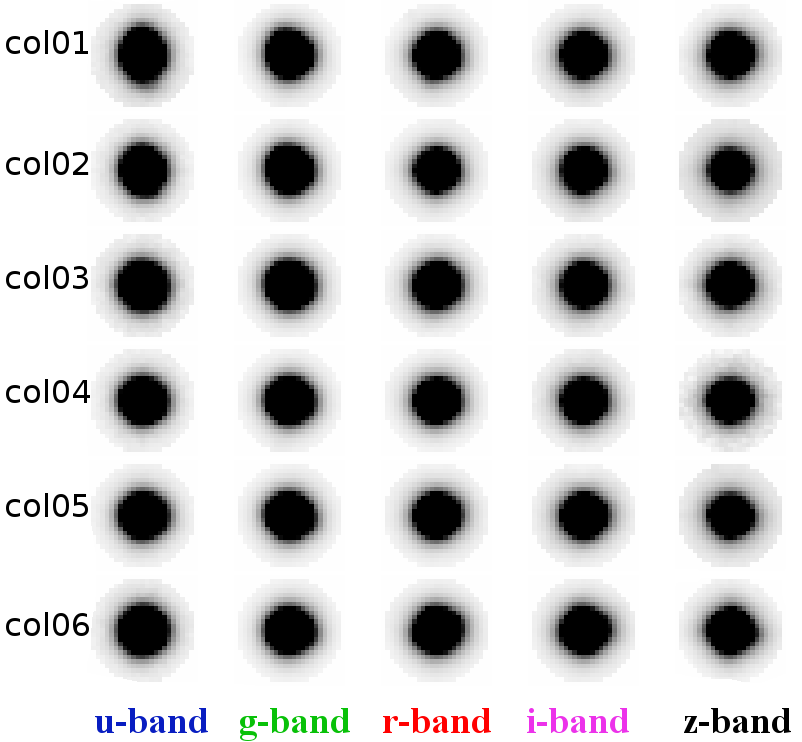
\includegraphics[width=6in]{Figures/psf_allbands_6cols.png}
\caption{A set of PSFs for five bands for odd columns centered at RA=21:56:46. All PSFs are scaled to the unit flux}
\label{fig:psf}
\end{figure}

We used {\tt IRAF/lucy}, a task that uses algorithm developed independently by Lucy \citep{Lucy1974} and Richardson \citep{Richardson1972}, to create kernels for pairs of images in x- and u-bands, where "x-" stands for g-, r-, i-, or z-band. 
Parameters  for {\tt IRAF/lucy} :\\
\begin{tt}
input  = u-band PSF\\ 
psf    = g-, r-, i-, or z-band PSF\\ 
niter  =  50\\ 
limchis=  $1.0E-14$\\ 
accel\_m=  standard\\ 
	\end{tt}

With kernels in hand it is now possible to run {\tt IRAF/psfmatch} that convolves input image with the kernel to produce a psf matched output image (Figure~\ref{fig:psfmatch}). 
Parameters  for {\tt IRAF/psfmatch} :\\
\begin{tt}
input = g-, r-, i-, or z-band FITS  file\\ 
kernel = kernel.fits\\ 
output = x\_matched\_u.fits\\ 
convolu = kernel\\ 
	\end{tt}

\begin{figure}[!ht]
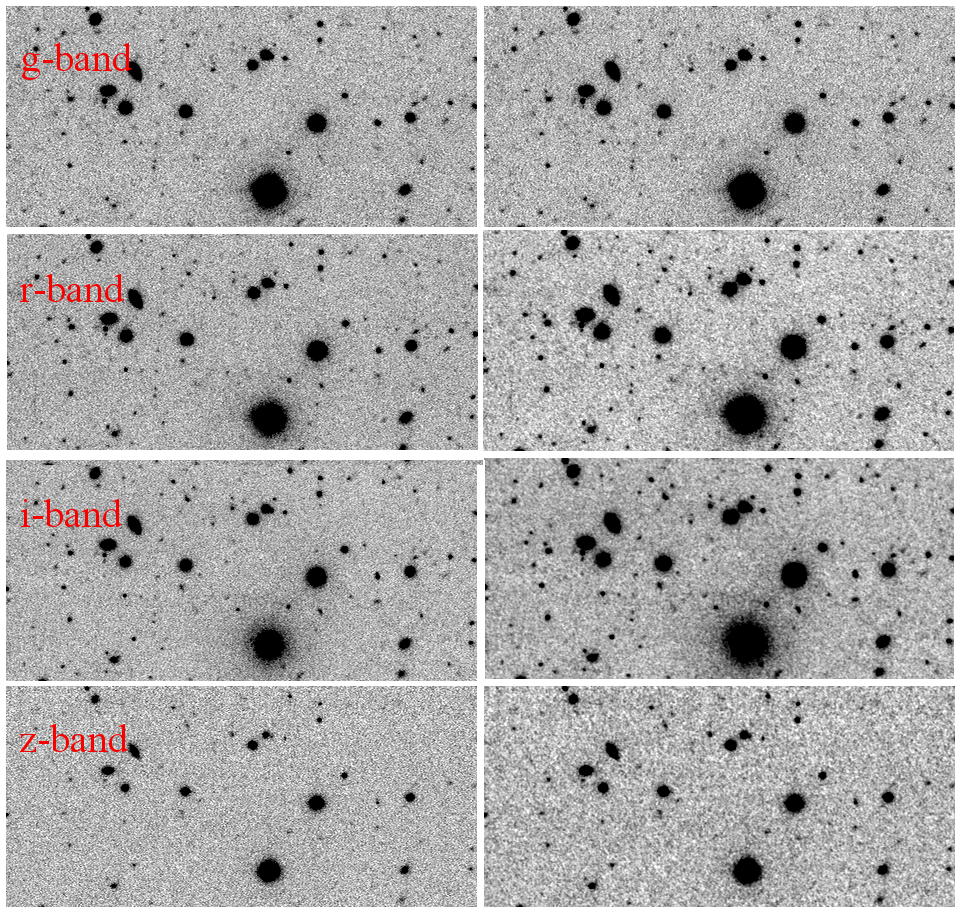
\includegraphics[width=6in]{Figures/psfmatch.png}
\caption{An example of {\tt IRAF/psfmatch} for $griz$ bands (top to bottom). Original images are to the left, PSF-matched - to the right. The difference is mostly observable for r- and i-bands, because their  PSF is much better than that of the u-band}
\label{fig:psfmatch}
\end{figure}


\subsection{Construction of the optical part of the catalog}
As outlined above, different bands have different sensitivity and FWHM, so faint sources may not be detected in all bands. In order to construct our catalogs we ought to select one band as the detection band. It has to be deep enough to have as many sources as possible and also has good FWHM to constrain the shape of the sources - that is crucial for the flux measurement in unWISE bands as each image must be supplied to {\tt TPHOT} along with the corresponding segmentation file and also each source in the catalog must have its x\_min, x\_max, y\_min and y\_max vales. As can be seen on Fig.9 from J14, $riz$ bands have the best FWHM out of 5 bands, and among them r-band has the highest limiting magnitude (24.6, comparing to 24.1 and 22.8 AB magnitudes in i- and z-band respectively). We choose r-band to be the base catalog of our sample and we used position of the source in this band to extract flux in $ugiz$ bands in SDSS and also in w1 and w2 bands of unWISE images.

Now we run {\tt SExtractor} in the dual mode (the first image is used for detection and astrometry information, while the second is used solely for photometry) to create a 5-band optical catalog. We use r\_matched\_u images for the detection of sources and x\_matched\_u image for the photometry, (u\_matched\_u is just u-band image). All bands are PSF matched to the u-band, and thus the same FWHM so {\tt SExtractor} parameters are identical with the exception of the magnitude zeropoint. Complete list of parameters is provided in \hyperref[sec:sex]{Appendix}. As the next step we reject sources with SNR $<5$ based on the r\_matched\_u flux. We notice that very few sources were rejected at this stage - objects that appear almost undetectable had FLUX\_AUTO / FLUXERR\_AUTO larger than 5 or even 7. We address this issue in the next section, and note that we decide not to reject those sources and supply it to {\tt TPHOT} because we shall use residual images to detect "WoDrops" - objects that are undetectable in optical bands. i.e., dropouts. But for the purpose of the GSMD construction we corrected magnitude errors and rejected sources with SNR $<5$ before starting the SED fitting.

\subsection{Magnitude error correction}

Photometry comparison between original x-band and x$\_$matched$\_$u-band catalogs shows a systematic underestimation of the errors associated with the sources' flux (Figure~\ref{fig:err_corr}). To correct for that we use {\tt STILTS} code \citep{Taylor2006} to match x-band and x$\_$matched$\_$u catalogs in 5 bands and for each separate image we calculate the mean ratio of the flux error before and after PSF. 
All magnitude errors in a given image are then multiplied by this coefficient. This correction coefficient can also be used as a test of our PSFs - all coefficients should occupy a narrow region with values within 1.2-2.2 for $griz$ bands with very few outliers (Figure~\ref{fig:err_corr_coef}).
We did not apply {\tt IRAF/psfmatch} task to the u-band, but still calculated that correcting coefficient because r\_matched\_u FITS file was used as detection image in {\tt SExtractor}. All coefficients for this band are less than 1. 

\begin{figure}[!ht]
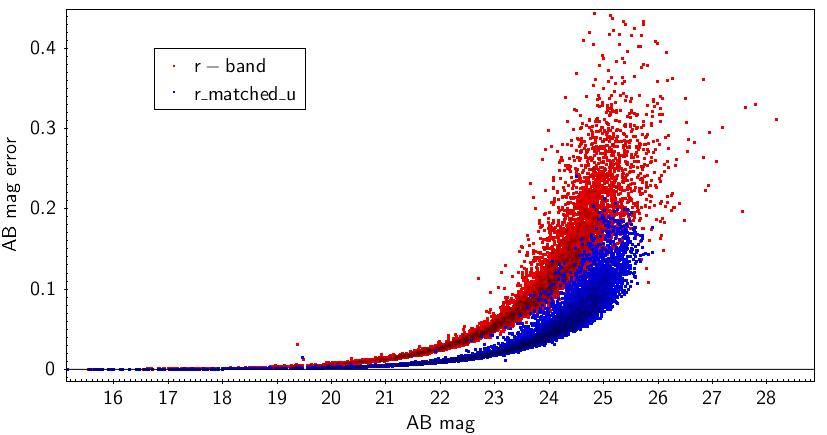
\includegraphics[width=6in]{Figures/error_correction_rband_example.jpg}
\caption{An example of the change in magnitude error for r-band photometry. Original errors are plotted against AB mag in red, magnitude errors \textit{for the same source} after {\tt IRAF/psfmatch} is performed are in blue.}
\label{fig:err_corr}
\end{figure}

\begin{figure}[!ht]
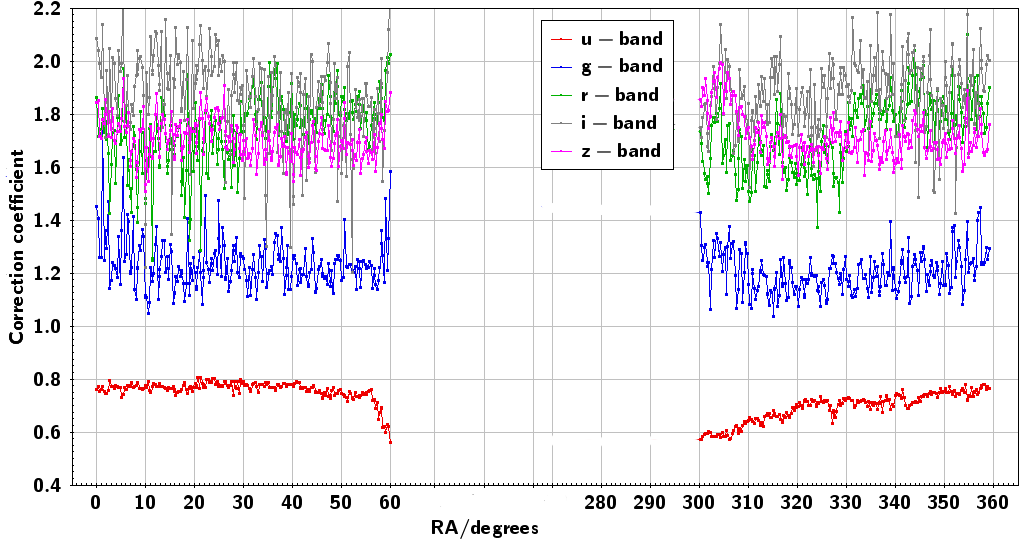
\includegraphics[width=6in]{Figures/magerr_corr_04.png}
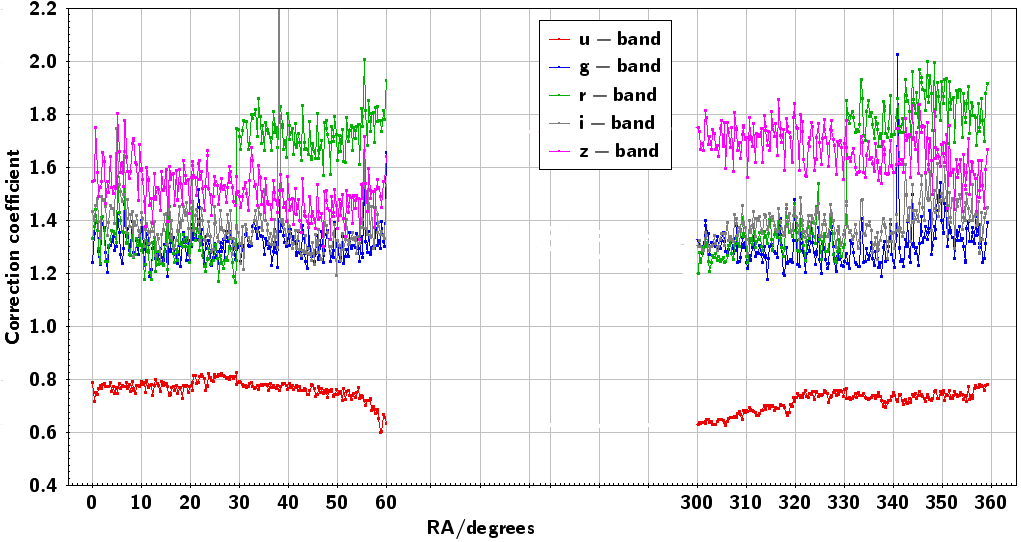
\includegraphics[width=6in]{Figures/magerr_corr_12.png}
\caption{Correction coefficients for all 5 bands for two columns - col04 (top) and col12 (bottom). Note that coefficients for the u-band are less than one}
\label{fig:err_corr_coef}
\end{figure}

We anticipate that while corrected values account for statistical error, there should also be a systematic error in magnitude that needs to be taken care of. We performed a series of tests where different constant errors were added in quadrature to the reported magnitude error and then the goodness of fit on the graph z\_spec vs z\_phot was checked. We found that correlation is the tightest when 0.04 magnitude error is added in quadrature (so final error cannot be smaller than 0.04). So finally, each source in each band was assigned by a error in magnitude that was calculated using the following equation: 
$$ magerr\_corrected = \sqrt{0.04^{2}+(\dfrac{1.0857}{SNR}\cdot correction\_coefficient)^{2}}$$

At this point construction of the optical part of the sample is complete. Our parent catalog now consists of 26,585,000 sources. 

\section{Preparatory work with unWISE files}
	{\tt TPHOT} is very demanding to the quality of the input files, any small variation severely skews results, so we pay particular attention to this part.
	
\subsection{unWISE PSF construction}
	
We use {\tt SWarp} to change the pixel scale of all unWISE images from original 2.75 to 2.772 to match the integer pixel scale ratio with SDSS images $\dfrac{2.772}{0.396}=7$. Now we construct unWISE PSF functions that is to be convolved with SDSS PSF to produce kernels - one of the most important set of the input files to {\tt TPHOT}. There are 240 unWISE images within Stripe 82 footprint per band. Bands w3 and w4 are too shallow and no reasonable flux can be extracted for the vast majority of optical sources  in these bands, so for the purpose of this project we only use w1 and w2 bands. That means we need to make another 480 PSFs.
We followed the strategy from the previous section to construct PSF for all 480 images (i.e., running {\tt SExtractor}, selecting potential PSF stars using {\tt STILTS}) with two major differences in the procedure:\\
1) Center pixels of saturated sources in unWISE standard deviation images (unwise-0000p000-w1-std-m.fits) always have zero value and that is an invalid input for {\tt TPHOT}. We use {\tt IRAF/imcalc} to detect such pixels and change its value to "9999".\\
2) We construct each PSF function manually, using {\tt IRAF/psf} in interactive mode. This was done to perform more robust selection of stars as 3 PSFs from one unWISE frame are convolved with 72 SDSS PSFs and thus its quality is crucial - incorrect PSF profile leads to wrong flux estimation associated with such sources and also characteristic positive and negative ring-shaped patterns in the residuals. \\
After running the {\tt IRAF/seepsf} task we get PSF FITS images, 19x19 pixels each. All unWISE PSFs are then scaled to the unit flux with {\tt IRAF/imarith} and sub-sampled in size by the factor of 7 using {\tt IRAF/imlintran} (to 133x133 pixels) to match the pixel scale ratio between unWISE and SDSS images. Result is presented on Figure~\ref{fig:unwise_psf}

\begin{figure}[!ht]
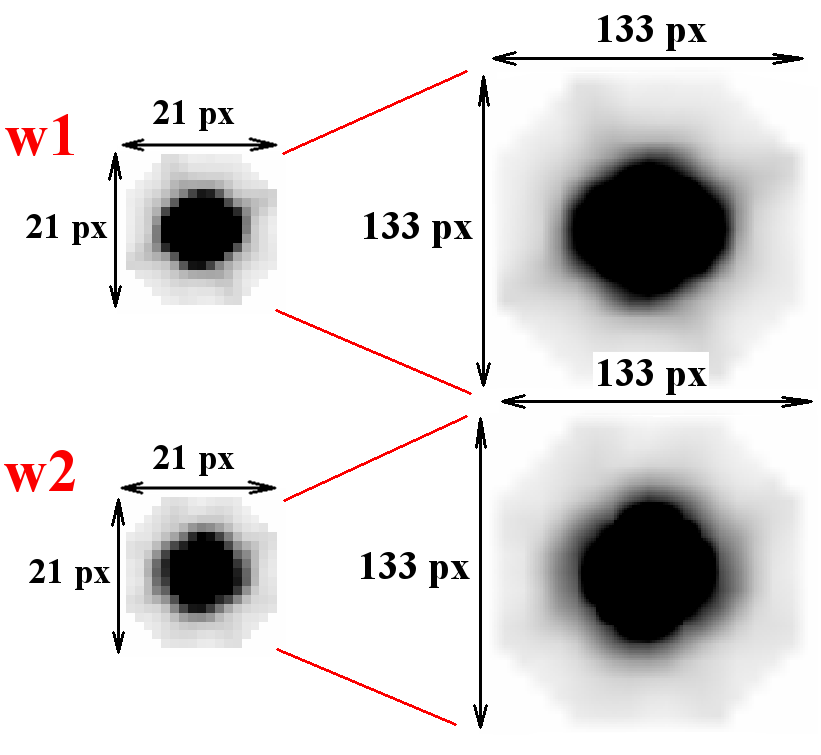
\includegraphics[width=6in]{Figures/unwise_psf.png}
\caption{unWISE PSFs for w1 (top row) and w2 bands (bottom row), as constructed in {\tt IRAF/psf} (left) and scaled by factor x7 to mimic pixel scale ratio between SDSS and unWISE pixel scales (right)}
\label{fig:unwise_psf}
\end{figure}

\subsection{Naming convention for the processed files}

Both final and intermediate results are a combination of SDSS and unWISE data and we introduce our naming convention that is used throughout the project. E.g. file
kernel.w1.0000p015\_12r\_u\_111.fits is a kernel made by convolution of the PSF function of the file unwise-0000p015-w1-img-m.fits and PSF function of the file S82\_12r\_111.fits in r-band, that has been previously matched to the PSF of the u-band.


\section{Template fitting with {\tt TPHOT}}
{\tt TPHOT} is a software designed to perform a precision photometry on a low-resolution images using information provided by a high-resolution images of the same field. Running {\tt TPHOT} on such a large portion of the sky with individual kernels for every pair of high- and low-resolution image is a key feature of our project.

In order to get the best results we follow recommendations of E.Merlin and perform two runs ("pass 1" and "pass 2") of {\tt TPHOT} on each pair (low- and high-resolution) of images. The second pass is performed using local kernels registered after the shifts in x and y coordinates are determined in the first pass.

One of the advantages of {\tt TPHOT} is a large saving of computational time comparing to its forerunners, {\tt TFIT} or {\tt CONVPHOT} codes, but it still needs lots of CPU time. Each SDSS image has on average 5200 sources and each pass of {\tt TPHOT} takes $\sim3$ hours CPU time. We perform template fitting on two unWISE bands so the total number of passes is $5556 \cdot 2 \cdot 2$ that requires $\approx 66,700$ CPU hours. We use our access to the University of Missouri High-Performance Computing (HPC) cluster ”Lewis” to process all images.

There are six different files supplied as an input to each run of {\tt TPHOT}:\\
-	High-resolution image - SDSS r-band FITS image matched to the u-band PSF\\
-	Source catalog with position, flux and background measurements for each source\\
-	Segmentation map corresponding to the SDSS image and having the value of the id of each source in the pixels belonging to it, and zero everywhere else\\
-	Low-resolution image - unWISE either w1 or w2 FITS image\\
-	Low-resolution weight image\\
-	kernel - result of convolution of high- and low-resolution PSFs\\

Dimensions of high- and low-resolution images do not have to be the same for successful run of {\tt TPHOT}, so generally we can supply full unWISE frame as the low-resolution image, but the code performs certain mathematical operations on such image during each pass, and such operations are mutually interfering when one tries to simultaneously run {\tt TPHOT} on several SDSS images that belong to the same unWISE frame. In order to run several {\tt TPHOT} jobs at the same time at Lewis cluster we created 18.828'x13.523' unWISE cutouts (with associated weight image) for each SDSS image.

After considerable number of test runs we came up to the following set of parameters that provides us with the best results. We only list the most important parameters here, full list is available in \hyperref[sec:tphot]{Appendix}:\\
{\tt order standard 			}$\#$ Used for the first pass\\
{\tt order standard2 		}$\#$ Used for the second pass\\
{\tt usereal         True    }$\#$ Real 2-d profiles\\
{\tt relscale        7		}$\#$ Pixel ratio between detection and measure image\\
{\tt FFTconv         true 	}$\#$ Use FFT for convolution of cutouts\\
{\tt fitting         single	}$\#$ One of three possible fitting methods\\
{\tt fitbackground   false}\\
{\tt clip            true 	}$\#$ Clip out large negative fluxes and re-do the fit\\
{\tt dzonesize       5 		}$\#$ Pixels size of region in which PSF shift is computed\\

\subsection{{\tt TPHOT} output files}

The most important {\tt TPHOT} output files are low-resolution residual FITS image, which is obtained by subtracting the model image from the low-resolution image, and catalog of residual fluxes and corresponding flux errors for each input source that was successfully fitted. {\tt TPHOT} rejects source if it lies outside of the low-resolution frame or if it has too high RMS. For such rejected source the fitted flux and flux errors are assigned to be $-99$ and $99.0E8$ respectively - such source is still used for SED fitting and we do not create any special subsample for the sources without near-IR photometry. On Figure~\ref{fig:resid} three images are shown - r-band SDSS, w1-band unWISE and residual in w1-band. Red circles with 3" radius are drawn around optical sources that are supplied to {\tt TPHOT}.

\begin{figure}[!ht]
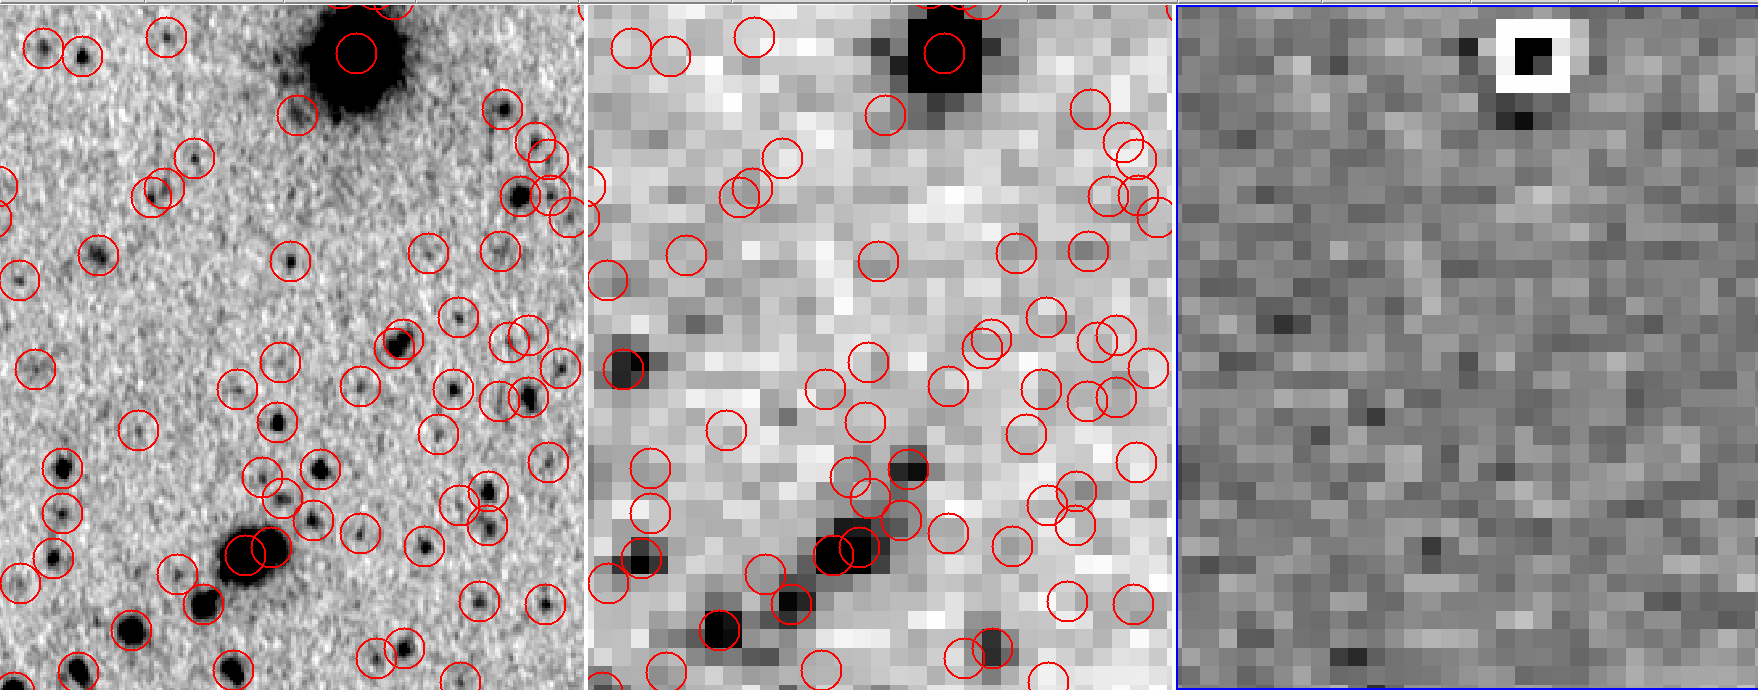
\includegraphics[width=6in]{Figures/sdss_unwise_resid.png}
\caption{From left to right: SDSS image in r-band, unWSIE w1 image, residual image from {\tt TPHOT}. SDSS sources that are fitted to the unWISE image for the flux estimation are denoted with red circles. These objects are cleaned out from the residual image}
\label{fig:resid}
\end{figure}


\section{Matching optical and IR catalogs}

Once all unWISE images within Stripe 82 footprint in w1 and w2 bands are processed by {\tt TPHOT}, output catalogs need to be matched with optical ones. Matching is performed with {\tt STILTS} code by using the source ID as the parameter to match. Additional test is performed in order to verify that photometry in optical and IR indeed belongs to the same source: difference in r-band {\tt FLUX$\_$ISO} and {\tt TPHOT} input flux in both bands is calculated and it should be zero.

As the next step fluxes in the matched catalogs are converted from counts/sec to AB magnitudes and flux in microJansky.
